\documentclass[aima331_lecturenotes_ku.tex]{subfiles}

\begin{document}
\chapter*{Vector Calculus Continued...}

The vector integral calculus extends integrals as known from calculus to integrals over curves (``line integrals''), surfaces(``surface integrals''), and solids. The known integral from calculus is the theory of integration over coordinate lines and planes which is extended in vector calculus to general curves and surfaces in space. We shall see that these integrals have basic engineering applications in solid mechanics, in fluid flow, and in heat problems.

\section{Integral of Vector Function}
The indefinite integral of $\vec{r}$ with respect to $t$ is given by:
$$\int \, \vec{r}(t)\,dt = \vec{R}(t) + C$$
If the components of $\vec{r}=f(t)\hat{i} + g(t)\hat{j}+h(t)\hat{k}$ are integrable over $[a,b]$, then so is $\vec{r}$, and the definite integral of $\vec{r}$ from $a$ to $b$ is
$$\int_{a}^{b} \; \vec{r}(t)\,dt = \int_{a}^{b}\,f(t)\,dt\,\hat{i} + \int_{a}^{b}\,g(t)\,dt\,\hat{j} + \int_{a}^{b}\,h(t)\,dt\,\hat{k}$$

\section{Line Integrals}
To calculate the total mass of a wire lying along a curve in space, or to find the work done by a variable force acting along such a curve, we need more general notion of integral. We need to integrate over a curve $C$ rather than over an interval $[a,b]$.

The concept of a line integral is a simple and natural generalization of a definite integral $\displaystyle \int_a^b \; f(x)\, dx$, known from calculus. In this definite integral we integrate the $f(x)$ from $x=a$ to $x=b$ along the $x-axis$. In a line integral we shall integrate a given function, along a \textbf{curve C} in a space or in the plane. Hence \
\textit{curve integral} would be a better name, but line integral is standard. \\

\subsection{Line integral of scalar function}
Suppose $f(x,y,z)$ is a real-valued function (scalar function) that is to be integrated over the curve $C$ lying within the domain of $f$ and parametrized by $r(t) = x(t)\hat{i}+y(t)\hat{j} + z(t)\hat{k}, \;\; a \leq t \leq b$. The values of $f$ along the curve are given by the composite function $f(x(t),y(t),z(t)$. Then $ds=\sqrt{dx^2 + dy^2 + dz^2}$ is the small element of $C$. So, the line integral of $f$ over $C$ is
\begin{equation}
  \label{line_scalar}
  \int_C\, f(x,y,z)\,ds =     \int_a^b\, f(x(t),y(t),z(t))\,(ds/dt) dt
\end{equation}
where $ds$ is the small element of $C$, analogous to $dx$ as small element of the interval $[a,b]$ on $x-axis$. \textit{Thus we have converted the line integral into the ordinary definite integral}.

\subsection{General Assumptions}
\begin{itemize}
\item The curve $C$ is called the path of integration, $r(a)$ its initial point and $r(b)$ its terminal point. $C$ is now \textbf{oriented}.

\item The direction from $A$ to $B$, in which $t$ increases, is called the positive direction on $C$ and can be marked by an arrow. The points $A$ and $B$ can coincide, forming a closed path.

\item $C$ is \textbf{piecewise smooth} that is, it consists of finitely many smooth curves, or finitely many points where $r(t)$ is not differentiable or $r(t)$ is zero.  For example, the boundary of a square is piecewise smooth, consisting of four smooth curves (the four sides).
  \end{itemize}

\subsection{Line Integral of vector field}
A line integral of a vector function $F(r)$ over a curve $C:r(t)$ is defined by
\begin{equation}
  \label{line_vec}
  \int_C \, F(r).dr = \int_C \, F(r(t)).(dr(t)/dt)\;dt
\end{equation}
In cartesian coordinates $F=F_1\hat{i} + F_2\hat{j} + F_3\hat{k}$ and $dr=dx\hat{i} + dy\hat{j} + dz\hat{k}$, then the line integral~\ref{line_vec} becomes
\begin{equation}
  \label{line_cartesian}
\int_C \, F(r).dr = \int_C \, (F_1dx+F_2dy+F_3dz)
\end{equation}
If the path $C$ is a closed curve, then the symbol for line integral is $\displaystyle \oint_C$.

\subsection{Motivation of the Line Integral}
The work $W$ done by a constant force $F$ in the displacement along a straight segment $r$ is $\mathbf{W=F.r}$. For a variable force $F$ on a curve $C:r(t)$, we find a small work done, on small segment $dr$ by $F$ where, $F$ acts as constant on this segment $dr$. The small work done is $dW=F.dr$. The total work done is then $\mathbf{W=\int_C\, dW= \int_C \, F.dr}$. \\
So, the line integral in this case gives the total work done by the variable force $F$ acting on the path $C$. This practical motivation for the line integral.

\subsection{Exercise}
\begin{enumerate}
\item Calculate work done by the given force along the given path.
  \begin{enumerate}
  \item $F=(y^3, x^3)$,  $C$ is the parabola $:y=5x^2$ from $A=(0,0)$ to $B=(2,20)$.
  \item $F=(e^x, e^y)$, $C$ is circle with center $(0,0)$ from $(1,0)$ to $(0,-1)$, clockwise.
  \item $F=(e^x, e^y, e^z)$, $C:r=(t, t^2, t^2)$ from $(0,0,0)$ to $(2,4,4)$.
   \item Find the work done by the force field $\vec{F} = (y-x^2)\hat{i} + (z-y^2)\hat{j} + (x-z^2)\hat{k}$ along the curve $\vec{r}(t) = t\hat{i} + t^2\hat{j} + t^3\hat{k}$, from $(0,0,0)$ to $(1,1,1)$.
  \end{enumerate}
\end{enumerate}

\begin{figure}[h]
  \centering
  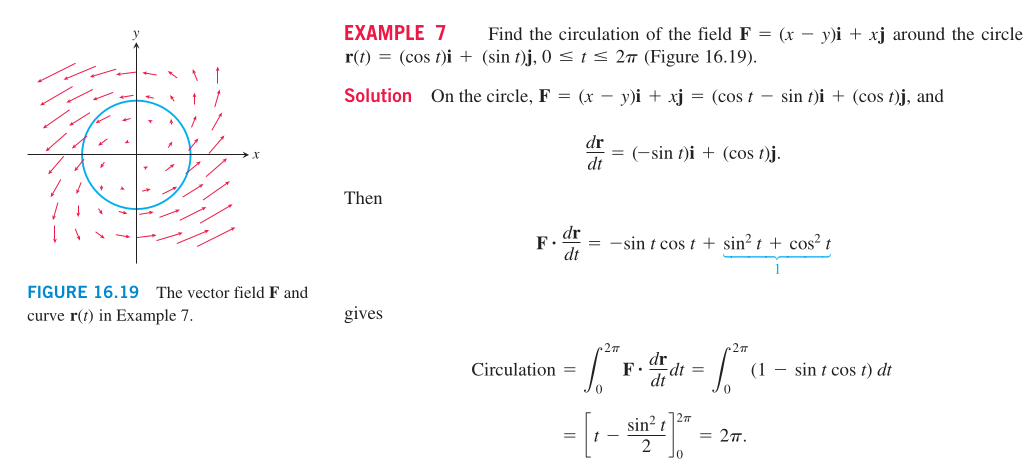
\includegraphics[width=16cm, height=8cm]{circulation.png}
\end{figure}

\subsection{Flow Integrals and Circulation}
Suppose that $\vec{F}$ represents the velocity field of a fluid flowing through a region in space. Under these circumstances, the line integral along a curve in the region gives the fluid's flow along, or circulation around, the curve. In this case the line integral is called a flow integral. And if the curve end and start at the same point then it is called a circulation.

\subsection{Flux Across a Simple Closed Plane Curve}
A curve in the $xy$-plane is simple if it does not cross itself. If $C$ is a smooth simple closed curve in the domain of a continuous vector field $\vec{F}$ in the plane, and if $n$ is the outward unit normal vector on $C$, the flux of $\vec{F}$ across $C$ is $\displaystyle \int_C\; \vec{F}.\vec{n}\;ds$


\subsection{Path Dependence}
\begin{theorem}
  The line integral generally depends not only on $F$ and on the endpoints $A$ and $B$ of the path path, but also on the path itself along with the integral is taken.
\end{theorem}
\begin{proof}
  Let us take two different curve $C_1: r_1(t)=(t,t,0)$ (straight line)  and $C_2:r_2(t)=(t,t^2,0)$ (parabola) on $[0,1]$. For $F=(0,xy,0)$, $F.dr_1 = t^2$ and $F.dr_2 = 2t^4$, so that integration becomes $1/3$and $2/5$, respectively.
\end{proof}

\subsection{Path Independence of Line Integrals}
In this sections we discuss the conditions for path independence of a line integral.
Let us consider a line integral
\begin{equation}
  \label{line_vec_cartesian}
  \displaystyle \int_C\, F(r).dr=\int_C\,(F_1dx + F_2dy + F_3dz)
\end{equation}
\begin{theorem}
  The line integral~\ref{line_vec_cartesian} with continuous components of the vector field $F=(F_1, F_2, F_3)$ in a domain $D$ in space is path independent in $D$ if and only if $F$ is the gradient of some function $f$ in $D$, i.e., $F=grad \,f$
\end{theorem}

\begin{theorem}
  The line integral~\ref{line_vec_cartesian} is path independent in a domain $D$ if and only if its value around every closed path in $D$ is zero.
\end{theorem}

\begin{theorem}
  The integral~\ref{line_vec_cartesian} is path independent in a domain $D$ if and only if the differential form $F_1dx + F_2dy + F_3dz$ is exact in $D$.
\end{theorem}

\subsection{Green's Theorem}
\begin{mdframed}
  Let $R$ be a closed bounded region in the $xy$-plane whose boundary $C$ consists of finitely many smooth curves. Let $F_1(x,y)$ and $F_2(x,y)$ be functions that are continuous and have continuous partial derivatives $\partial F_1 /\partial y$ and $\partial F_2 /\partial x$ everywhere in some domain containing $R$. Then
  \begin{equation}
    \label{green}
    \int \, \int _R \; \left ( \frac{\partial F_2}{\partial x} - \frac{\partial F_1}{\partial y}  \right )\;dx\,dy = \oint_C (F_1\,dx + F_2 \, dy)
  \end{equation}
\end{mdframed}
Here we integrate along the entire boundary $C$ of $R$ in such a sense that $R$ is on the left as we advance in the direction of integration.

\subsection{Exercise}
\begin{enumerate}
\item Prove that conservative vector field are irrotational vector field.
\item For the following vector-field are conservative vector field, and hence find a scalar function $f$ such that $F=\nabla f$.
  \begin{multicols}{3}
    a). $F=(yz,xz,xy)$
    \columnbreak

    b). $F=(2x,4y,8z)$
    \columnbreak

    c). $F(x^2-yz, y^2-zx, z^2-xy)$

  \end{multicols}
\item Use Green's theorem to evaluate $\int_C\, F(r).dr$.
  \begin{enumerate}
  \item $F=(xy^4,x^4y)$, $R$ the rectangle with vertices $(0,0), \; (3,0), \; (3,2), \; (0,2)$.
  \item $F=(x-y,x+y)$, $R$ the region bounded by $y=x^2$ and $y=\sqrt{x}$.
  \item $F=(2x-y+4,5y+3x-6)$, $R$ the region inside the circle $x^2+y^216$.
   \item $F=(x^3-3y,x+siny)$, $R$ the triangle with vertices $(0,0), \; (1,0), \; (0,2)$.
  \end{enumerate}
\end{enumerate}

\section{Surface Integrals}
Like line integrals, surface integrals arise in two forms. One form occurs when we integrate a scalar function over a surface, the second form is for surface integrals of vector fields. \\
To compute the mass of a surface, the flow of a liquid across a curved membrane, or the total electrical charge on a surface, we need to integrate a function over a curved surface in space. An example of this form occurs when we want to measure the net flow of a fluid across a surface submerged in the fluid.

\subsection{Surface Integrals of a vector field}
Let $F$ be a vector field in three-dimensional space with continuous components defined over a smooth surface $S$ having a chosen field of normal unit vectors $n$ orienting $S$. Then the surface integral of $F$ over $S$ is:
\begin{equation}
  \label{surf}
  \int\int_S \, F. \, \vec{d\sigma} \;\;= \;\; \int\int_S \, F. \hat{n}\, d\sigma
\end{equation}
where, $\vec{d\sigma}$ is the surface element $S$ that has direction towards its normal. \\[2mm]
The surface integral of $F$ is also called the \textbf{flux} of the vector field across the oriented surface $S$. If $F$ is a \textbf{velocity field} of a three dimensional fluid flow, then the flux $F$ across $S$ is the net rate at which fluid is crossing $S$ per unit time in the chosen positive direction $n$ defined by the orientation of $S$.

\subsection{Representations of Surfaces}
Surfaces in $xyz$-space have the following representations:
\begin{itemize}
\item Explicit representation: $z=f(x,y)$
 \item Implicit representation: $g(x,y,z)=0$
 \end{itemize}
 The parametric representation of a curve is a mapping of the interval $a\leq t \leq b$, located on the $t-axis$, onto the curve $C$ in $xyz$-space. Similarly, for surfaces $S$ the parametric representation will consists of two parameters $u$ and $v$, as surfaces are two-dimensional. Thus a parametric representation of a surface $S$ in space is of the form:
 \begin{equation}
   \label{par_surface}
 r(u,v)=(x(u,v), \; y(u,v), \; z(u,v))
\end{equation}
where $(u,v)$ varies in some region $R$ of the $uv$-plane.
\begin{itemize}
\item The parametric representation of a cylinder $x^2+y^2=a^2, \;\; -1 \leq z \leq 1$ is \\ $r(u,v)=(a\,cosu, \; a\,sinu, v)$.

\item The parametric representation of a sphere $x^2+y^2+z^2=a^2$ is \\ $r(u,v)=(a\,cosv\,cosu, \; a\,cosv\,sinu, asinv) $.
\end{itemize}
The partial derivatives, $r_u$ and $r_v$ at $P$ to the surface~\ref{par_surface} are tangential to the surface. We assume that they are linearly independent. Then $r_u$ and $r_v$ span the tangent plane of $S$ at $P$. Hence their cross product gives a \textbf{normal vector N} of $S$ at $P$.
  \begin{equation}
    \label{surf_normal}
    \vec{N} = r_u \times r_v \implies \hat{n} = \frac{\vec{N}}{|\vec{N}|} = \frac{r_u \times r_v}{|r_u \times r_v|}
  \end{equation}
  But for non-parametric representation of surface $g(x,y,z)=0$: $\displaystyle \hat{n}=\frac{\nabla g}{|\nabla g|}$.
  \begin{mdframed}
    The surface area differential for a parametrized surface is
    \begin{equation}
      \label{surface_diff}
      d\sigma = |r_u \times r_v|\;du\,dv = N\,du\,dv
    \end{equation}
  \end{mdframed}
  Because the surface element is a parallelogram, whose sides are the vectors: $du\,r_u$ and $dv\,r_v$. The area of this parallelogram is $d\sigma$.

  \subsubsection{Surface Integral a Non-parametrized surface}
  \begin{enumerate}
  \item For a scalar function: \\[1mm]
    $\displaystyle \int\int_S\, F\frac{|\vec{N}|}{|\vec{N}.\hat{k}|}\,dx\,dy$

      \item For a vector function: \\[1mm]
    $\displaystyle \int\int_S\, F.\hat{n}\;\frac{dx\,dy}{|\hat{n}.\hat{k}|} = \int\int_S\, F.\vec{N}\;\frac{dx\,dy}{|\vec{N}.\hat{k}|}$
  \end{enumerate}

  \begin{figure}[h]
  \centering
  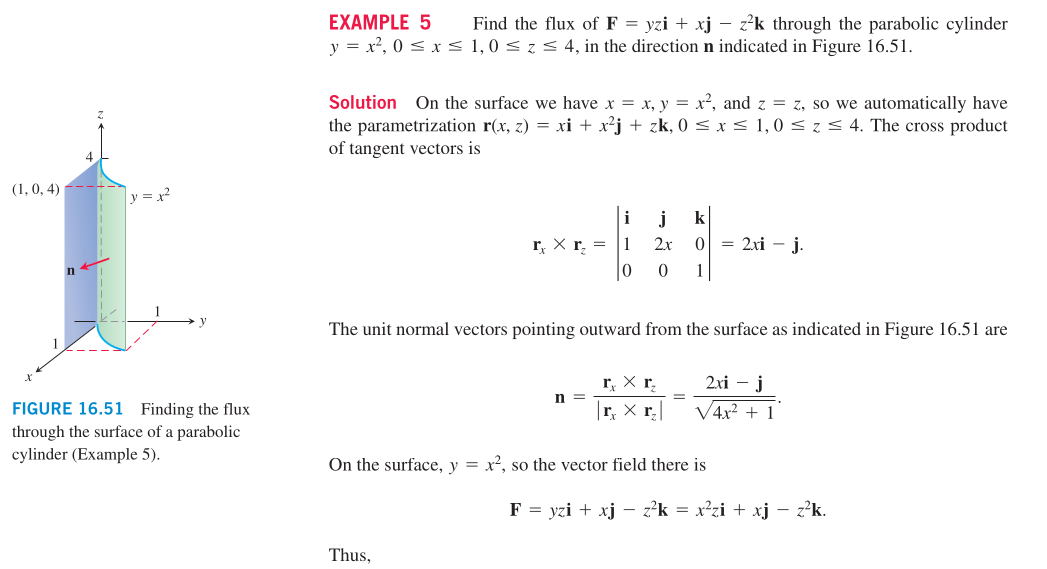
\includegraphics[width=16cm, height=8cm]{parasurface.png}
\end{figure}

\begin{figure}[h]
  \centering
  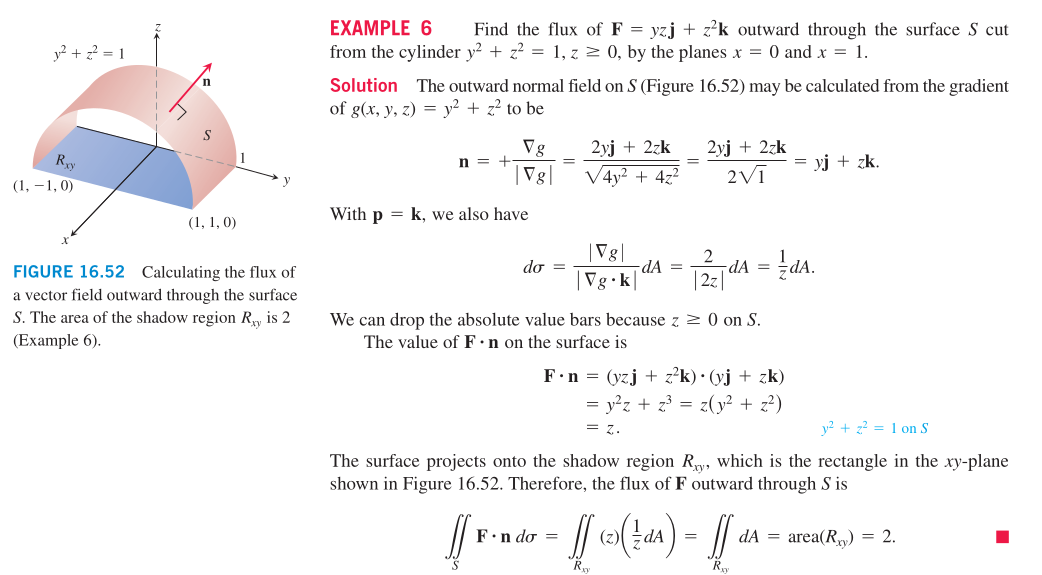
\includegraphics[width=16cm, height=9cm]{nonparasurface.png}
\end{figure}

  \section{Volume Integral}
  Volume Integrals are triple integrals. They can be transformed into surface integrals over the boundary surface of a region in a space and conversely. Such a transformation is of practical interest because one of the two kinds of integral is often simpler than the other.
  \begin{mdframed}
    \textbf{Divergence Theorem of Gauss} \\[1mm]
    Let $T$ be a closed bounded region in space whose boundary is a piecewise smooth orientable surface $S$. Let $F(x,y,z)$ be a vector function that is continuous and has continuous first partial derivatives in some domain containing $T$. Then
    \begin{equation}
      \label{divergence}
      \int \int \int _T div \, F \, dV= \int \int _S\, F.n\,d\sigma
    \end{equation}
  \end{mdframed}

  \subsection{Exercise}
  \begin{enumerate}
  \item Find the total mass of a mass distribution of density $\sigma$ in a region $T$ in space.
    \begin{enumerate}
    \item $\sigma = x^2y^2z^2$, $T$ the box $|x| \leq a$, $|y| \leq b$, and $|z| \leq c$.
     \item $\sigma = 1 + y+z^2$, $T$ the cylinder $y^2+z^2=9$, $1 \leq x 9$.
     \end{enumerate}

   \item Evaluate this integral by the divergence theorem.
     \begin{enumerate}
     \item $F=(x,y,z)$, $S$ the sphere $x^2+y^2+z^2 =9$.

     \item $F=(4x, 3z, 5y)$, $S$ the surface of the cone $x^2+y^2 \leq z^2$, $0\leq z\leq 2$.
     \end{enumerate}
  \end{enumerate}

\end{document}
%%% Local Variables:
%%% mode: LaTeX
%%% TeX-master: t
%%% End:
